\documentclass[conference]{IEEEtran}
\IEEEoverridecommandlockouts
% The preceding line is only needed to identify funding in the first footnote. If that is unneeded, please comment it out.
\usepackage{cite}
\usepackage{amsmath,amssymb,amsfonts}
\usepackage{algorithmic}
\usepackage{graphicx}
\usepackage{textcomp}
\usepackage{xcolor}
\usepackage{booktabs}

\def\BibTeX{{\rm B\kern-.05em{\sc i\kern-.025em b}\kern-.08em
    T\kern-.1667em\lower.7ex\hbox{E}\kern-.125emX}}

\begin{document}

\title{ROCKET: Exceptionally Fast and Accurate Time Series Classification Using Random Convolutional Kernels}

\author{\IEEEauthorblockN{Given Name Surname}
\IEEEauthorblockA{\textit{dept. name of organization (of Aff.)} \\
\textit{name of organization (of Aff.)}\\
City, Country \\
email address or ORCID}
\and
\IEEEauthorblockN{Given Name Surname}
\IEEEauthorblockA{\textit{dept. name of organization (of Aff.)} \\
\textit{name of organization (of Aff.)}\\
City, Country \\
email address or ORCID}
\and
\IEEEauthorblockN{Given Name Surname}
\IEEEauthorblockA{\textit{dept. name of organization (of Aff.)} \\
\textit{name of organization (of Aff.)}\\
City, Country \\
email address or ORCID}
\and
\IEEEauthorblockN{ Anton Lehnerer}
\IEEEauthorblockA{\textit{EHU} \\
alehnerer001@ikasle.ehu.eus}
}

\maketitle

\begin{abstract}
In this paper, we present ROCKET, a univariate time series classification algorithm based on random convolutional kernels, which combines speed and high accuracy. We evaluate ROCKET on a selection of datasets from the UCR repository and compare its performance against seven benchmark algorithms: 1NN-Euclidean, 1NN-DTW, Shapelet Transform, BOSS ensemble, Time Series Forest, InceptionTime and catch22. Our experimentation employs a robust validation framework and considers multiple evaluation metrics, including accuracy and computational efficiency. The results demonstrate that ROCKET consistently outperforms the benchmark algorithms in both accuracy and scalability, demonstrating its effectiveness for large-scale time series classification tasks.
\end{abstract}

\begin{IEEEkeywords}
time series classification, random convolutional kernels, ROCKET, benchmark
\end{IEEEkeywords}

\section{Introduction}
Time series classification is a fundamental task in many domains where large volumes of sequential data are generated and need to be processed efficiently and accurately. Examples include financial markets, healthcare and industrial monitoring. Traditional approaches often achieve competitive accuracy but suffer from high computational cost and limited scalability when applied to large or complex datasets.

ROCKET (RandOm Convolutional KErnel Transform) is an algorithm designed to overcome these limitations. It applies a large number of randomly initialized convolutional kernels to transform time series data into feature representations, which are then fed into linear classifiers. This approach enables both fast processing and high classification accuracy, even on large-scale datasets. 

In this paper, we evaluate ROCKET on a selection of UCR datasets and compare its performance with seven benchmark algorithms, analyzing both accuracy and computational efficiency.

\section{ROCKET Algorithm}
ROCKET transforms time series by applying convolutional kernels, which are not learned through training, but instead are randomly initialized. Each kernel has parameters including length, weights, dilation, and bias, all of which are assigned randomly. The randomness allows the algorithm to generate a diverse set of filters, capable of capturing a wide variety of temporal patterns. 

Once the kernels are applied to a time series, each convolution produces a feature map, showing the activation of the kernel across the entire series. From each feature map, ROCKET extracts two key summary features: Maximum value and Proportion of Positive Values (PPV).  

Using a large number of kernels, ROCKET transforms each time series into a high-dimensional feature vector, which captures a large variety of temporal patterns without requiring kernel training. 

These feature vectors are then fed into a linear classifier, typically Ridge Regression or Logistic Regression, which performs the final classification. 

\subsection{Kernels}
ROCKET relies on a large number of convolutional kernels to extract meaningful features from time series. Each kernel acts like a small filter that highlights certain patterns in the data. Although the kernels are randomly initialized and not learned, their diversity allows the algorithm to extract rich and varied features from the time series. This random initialization enables ROCKET to efficiently explore a wide variety of temporal patterns without the computational cost of training each kernel.

The main parameters of each kernel are:
\begin{itemize}
    \item \textbf{Length $l$}: determines how many consecutive points the kernels considers, which allows kernels of different scales to detect both short and long-term patterns.
    \item \textbf{Weights $w$}: sampled from a standard normal distribution, giving each kernel a unique pattern of emphasis over the input series.
    \item \textbf{Dilation $d$}: controls the spacing between points in the kernel. A dilation of $d > 1$ allows the kernel to skip points in the series, allowing the model to capture patterns that occur over longer time intervals or at multiple scales. 
    \item \textbf{Bias $b$}: random offset added to the convolution output, which increases the variability of the resulting feature map.
\end{itemize}
Additionally, padding is applied when necessary to ensure that kernels convert the full series, preserving feature extraction across all time points. Each kernel produces a feature map along the series, which will later be summarized in the feature extraction stage.

\subsection{Time series Transformation}
The core of the ROCKET algorithm lies in the transformation of the input time series via the application of the randomly generated convolutional kernels. Given a univariate time series $X = (x_1, x_2, \dots, x_n)$ and a random kernel with weights $W = (w_1, w_2, \dots, w_l)$, length $l$, dilation $d$, and bias $b$, the time series transformation is achieved through a 1D convolution operation. The kernel slides across the time series, computing the dot product between its weights and the corresponding subsequences of the input. Because of the dilation parameter $d$, the kernel does not necessarily interact with strictly contiguous data points; rather, it spans a receptive field of $(l - 1)d + 1$. For a specific position $i$ in the time series, the convolution output (activation) is calculated as:
$$a_i = \left( \sum_{j=0}^{l-1} x_{i+(j \cdot d)} \cdot w_{j+1} \right) + b$$
This operation is repeated across the entire sequence, producing a resulting vector known as a feature map, $M$. This map represents the degree to which the specific temporal pattern defined by the random kernel is present at each point in the time series. By applying a large ensemble of these kernels (typically 10,000 in the default configuration), ROCKET projects the original time series into a highly diverse, transformed spatial representation.

\subsection{Feature Extraction}
Passing the time series through 10,000 kernels results in 10,000 distinct feature maps. To make this high-dimensional output usable for a standard classifier without causing a combinatorial explosion in memory and processing time, ROCKET applies a pooling step to extract fixed-length scalar summaries from each feature map. For every feature map $M$, ROCKET extracts exactly two aggregate features: Maximum Value (Max): This captures the peak activation of the kernel across the entire time series. It acts as an indicator of the single strongest match between the kernel's pattern and the input data.
$$Max(M) = \max_i(M_i)$$
Proportion of Positive Values (PPV): This represents the frequency with which a pattern appears in the time series. It calculates the fraction of the feature map where the activation is strictly greater than zero.
$$PPV(M) = \frac{1}{|M|} \sum_{i=1}^{|M|} [M_i > 0]$$
(where $[ \cdot ]$ represents the Iverson bracket, equating to 1 if the condition is true and 0 otherwise). By extracting two features per kernel, an ensemble of 10,000 kernels produces a final, flat feature vector of 20,000 dimensions for each time series. This extraction mechanism is critical, as it allows ROCKET to handle input series of varying lengths while still outputting a uniform feature vector size for the classifier.

\subsection{Classifier}
Once the feature extraction phase is complete, the time series classification problem is effectively reduced to a standard tabular machine learning task. The 20,000-dimensional feature vectors are used to train a linear classifier. ROCKET typically employs a Ridge Regression classifier (for smaller datasets) or Logistic Regression (for larger datasets). The choice of a linear model is highly intentional: linear classifiers scale exceptionally well to high-dimensional data and are extremely fast to train. Because the random convolutional kernels combined with the non-linear PPV feature extraction inherently map the data into a space where the classes are largely linearly separable, complex non-linear classifiers (like deep neural networks or complex tree ensembles) are unnecessary. This synergy between diverse, random feature generation and a fast linear backend is the primary driver of ROCKET's computational efficiency.

\subsection{Advantages}
The ROCKET algorithm introduces several distinct advantages over traditional time series classification methods:
\begin{itemize}
    \item \textbf{Exceptional Computational Efficiency:} By eliminating the need to update kernel weights via gradient descent, ROCKET dramatically reduces training time. It achieves state-of-the-art accuracy in a fraction of the time required by deep learning models like InceptionTime or ensemble methods like HIVE-COTE.
    \item \textbf{High Accuracy:} Despite its reliance on random initialization, the sheer volume and diversity of the kernels allow ROCKET to capture a highly discriminative feature set, consistently matching or outperforming computationally heavier benchmarks.
    \item \textbf{Scalability:} The linear nature of the classification phase and the independence of the kernel convolutions make ROCKET highly scalable to both long time series and datasets with massive sample sizes.
    \item \textbf{Robustness to Hyperparameters:} ROCKET requires almost no hyperparameter tuning. The default setting of 10,000 kernels is universally effective across diverse domains, removing the need for costly cross-validation searches.
\end{itemize}

\subsection{Limitations}
While highly effective, the original ROCKET algorithm does have specific constraints:
\begin{itemize}
    \item \textbf{Memory Consumption:} Although computationally fast, storing the 20,000-dimensional feature vectors for every sample in a large dataset can lead to substantial RAM usage, which can be a bottleneck on memory-constrained hardware.
    \item \textbf{Lack of Interpretability:} Due to the random nature of the convolutional kernels, ROCKET acts largely as a "black box." It is exceedingly difficult to trace back exactly which temporal patterns or physical phenomena in the raw data drove the model's final classification decision.
    \item \textbf{Non-Determinism:} The random sampling of weights, biases, and dilations means that feature spaces will vary slightly between runs unless a strict random seed is applied, which can complicate exact reproducibility in some deployment environments.
    \item \textbf{Univariate Constraint:} The base ROCKET algorithm is designed explicitly for univariate time series, requiring architectural modifications (such as those seen in MultiROCKET) to effectively process multivariate data without losing cross-channel context.
\end{itemize}

\section{Variants}
Since its introduction, ROCKET has inspired a family of successors that address its main limitations—computational overhead, non-determinism, and restriction to univariate input—while preserving or improving upon its accuracy. The three principal variants are described below.

\subsection{MiniROCKET}
MiniROCKET (Dempster et al., 2021), optimizes the original framework by over an order of magnitude in computational speed without compromising classification accuracy. This variant transitions the model toward a nearly deterministic state by eliminating several stochastic components. In MiniROCKET, the kernel length is standardized to a fixed value of 9, and the weight space is constrained to only two discrete values. Unlike the original random initialization, the bias values are systematically derived from the distribution of the convolution outputs on the training data. Furthermore, the feature set is streamlined by discarding the "max" pooling operation, extracting only the Proportion of Positive Values (PPV). These structural constraints enable hardware-level optimizations that exploit the fixed parameters, providing a substantial reduction in training and inference latency while maintaining state-of-the-art performance across the UCR archive.

\subsection{MultiROCKET}
MultiROCKET, extends the framework to multivariate time series and introduces a significantly richer feature vocabulary. While maintaining the efficient weight scheme of MiniROCKET (utilizing the fixed pool of 84 binary vectors), MultiROCKET augments the feature extraction process by introducing three additional pooling operators beyond the original PPV and Max:
\begin{itemize}
    \item \textbf{Mean of Positive Values (MPV):} Captures the average activation strength, quantifying the intensity of a pattern match.
    \item \textbf{Mean of Indices of Positive Values (MIPV):} Encodes temporal localization by identifying where in the series a pattern typically occurs.
    \item \textbf{Longest Stretch of Positive Values (LSPV):} Measures the temporal persistence of a pattern through its longest contiguous activation.
\end{itemize}
These five operators produce $5 \times k$ features per channel, providing the linear classifier with critical information regarding the frequency, strength, location, and duration of detected patterns. For multivariate data with $C$ channels, the transformation is applied independently to each channel and concatenated. This approach achieves a statistically significant improvement in mean rank across the UCR archive while preserving a linear computational complexity of $O(k \cdot n \cdot l \cdot C)$. By avoiding cross-channel combinatorial kernels, MultiROCKET remains highly scalable while capturing a more comprehensive representation of complex temporal dynamics.

\subsection{Hydra}
Hydra introduces a dictionary-based approach using random convolutional kernels. Instead of relying on scalar pooling statistics, Hydra groups $g$ kernels with identical dilation and padding to construct a histogram of nearest-kernel assignments across the time series. This method acts as a highly efficient, randomized soft codebook—conceptually similar to the Bag-of-SFA-Symbols (BOSS) representation, but without the quadratic computational bottleneck of discretisation. This histogram-based representation excels at capturing the positional frequency of matched patterns, making it particularly effective for long and complex series.

Building upon this foundational concept, the Hydra-MultiROCKET architecture unites these methodologies by concatenating Hydra’s symbolic frequency histograms with the rich statistical pooling features of MultiROCKET. By simultaneously capturing the positional distribution of patterns (via Hydra) alongside their activation strength, duration, and temporal localization (via MultiROCKET), this combined variant achieves the highest mean classification accuracy within the ROCKET framework on the UCR archive to date. Furthermore, it maintains this state-of-the-art performance while operating an order of magnitude faster than deep learning baselines such as InceptionTime.

\section{Experimentation Comparison with Benchmark Models}
\subsection{Datasets}
We try to choose datasets from a range of different domains. In total, we include datasets from 9 different domains in our experimentation. The selection includes device/energy monitoring (Computers), biomedical signals (ECG200, EMOPain), industrial sensors (FordA, Earthquakes, Trace), spectroscopy (EthanolLevel, Beef), biology/motion capture (Worms, WormsTwoClass), image (SwedishLeaf, MiddlePhalanxOutlineCorrect), traffic (Chinatown), and synthetic benchmarks (CBF, SyntheticControl). We also take into account the length of the time series contained in the datasets. The lengths range from 24 (Chinatown) to 1751 (EthanolLevel). Dataset size: Since we do not use the predefined train/test split, we are interested in the total number of samples in the datasets. These span over a range of 60 (Beef) to 5000 (TwoPatterns). We also aim to reach a broad range of classes: Our selection mainly covers 2-class datasets, but we also include datasets with 3-6 classes (Worms, EMOPain, EthanolLevel, CBF, SyntheticControl, Beef, Trace). We also include a 15 class dataset (SwedishLeaf). We also try to include datasets with different difficulties. SwedishLeaf has 15 classes which are perfectly balanced, which makes the dataset overall more challenging for classification. On the contrary, we also include unbalanced datasets like Earthquakes. Notably, EMOPain is the only multivariate dataset in our selection (30 channels), which allows us to assess algorithm support for multivariate input.

\begin{table}[htbp]
\caption{Benchmark Datasets Description}
\label{tab:datasets}
\begin{center}
\resizebox{\columnwidth}{!}{
\begin{tabular}{lcccccccc}
\toprule
\textbf{Dataset} & \textbf{Train} & \textbf{Test} & \textbf{Total} & \textbf{Len.} & \textbf{Ch.} & \textbf{Cls.} & \textbf{Maj.} & \textbf{Domain} \\
\midrule
Computers & 250 & 250 & 500 & 720 & 1 & 2 & 0.500 & DEVICE \\
MiddlePhalanx & 600 & 291 & 891 & 80 & 1 & 2 & 0.622 & IMAGE \\
WormsTwoClass & 181 & 77 & 258 & 900 & 1 & 2 & 0.578 & MOTION \\
Worms & 181 & 77 & 258 & 900 & 1 & 5 & 0.422 & MOTION \\
Earthquakes & 322 & 139 & 461 & 512 & 1 & 2 & 0.798 & SENSOR \\
EMOPain & 968 & 355 & 1323 & 200 & 30 & 3 & 0.772 & HAR \\
EthanolLevel & 504 & 500 & 1004 & 1751 & 1 & 4 & 0.251 & SPECTRO \\
Chinatown & 20 & 343 & 363 & 24 & 1 & 2 & 0.713 & TRAFFIC \\
ECG200 & 100 & 100 & 200 & 96 & 1 & 2 & 0.665 & ECG \\
CBF & 30 & 900 & 930 & 128 & 1 & 3 & 0.333 & SIMULATED \\
SwedishLeaf & 500 & 625 & 1125 & 128 & 1 & 15 & 0.067 & SIMULATED \\
SyntheticControl & 300 & 300 & 600 & 60 & 1 & 6 & 0.167 & SIMULATED \\
Beef & 30 & 30 & 60 & 470 & 1 & 5 & 0.200 & SPECTRO \\
Trace & 100 & 100 & 200 & 275 & 1 & 4 & 0.250 & SENSOR \\
TwoPatterns & 1000 & 4000 & 5000 & 128 & 1 & 4 & 0.261 & SIMULATED \\
\bottomrule
\end{tabular}
}
\end{center}
\end{table}


\subsection{Evaluated Algorithms}
To evaluate our algorithm, ROCKET and its variations MiniROCKET, MultiROCKET and MultiROCKETHydra, we run experiments with seven benchmark classifiers. We include simple distance based classifiers, which classify by Nearest Neighbour, using Euclidian Distance (1NN-ED) and Dynamic Time Warping (1NN-DTW). From the shapelet based algorithms, we select Shapelet Transform (ST). We also include a dictionary based classifier with BOSS. We also choose Time Series Forest (TSF), which takes an interval based approach and a feature based classifier with catch22. Lastly, we include InceptionTime, a deep learning model. All classifiers are loaded from the aeon toolkit and run with default parameters. The only exception is InceptionTime. For computational feasibility, we adjust the number of training epochs to 100 (default is 1500). 

\subsection{Validation framework and metrics}
To ensure results that are robust, we evaluate all named algorithms with stratified 5-Fold Cross Validation. After loading the datasets from the UCR archive via aeon, we merge the train and test set. After, we repartition the samples and ensure that the classes are in equal proportion across the splits. For reproducibility, we fix the random seed to 42. 

The Performance was measured by using four metrics: accuracy, balanced accuracy, weighted F1-score and Cohen’s kappa. For datasets with a significant class imbalance, we are particularly interested in F1 score and Cohen's kappa. Additionally, we measure training and inference time. 

\subsection{Hardware}
To run our experiments, we distribute the experiments per dataset across different machines and then run the 5 folds for each classifier. We run the algorithms on CPU, with the only exception of InceptionTime, which is trained on GPU. For that, we use NVIDIA GeForce RTX 2080 GPUs. 

\section{Results}
\subsection{Classification Accuracy}
Table~\ref{tab:accuracy} reports the classification accuracy of each algorithm on all evaluated benchmark datasets. The best performance per dataset is highlighted in bold. Across the whole benchmark, MultiROCKETHydra achieved the highest mean accuracy of 0.909, followed by MultiROCKET at 0.908. MiniROCKET (0.895), ST (0.893), and ROCKET (0.888) reach very similar mean accuracy, while the distance-based baselines 1NN-DTW (0.791) and 1NN-ED (0.766) ranked the lowest. Shapelet Transform (ST) ranked fifth overall (0.893) but was the top performer on EthanolLevel---the hardest dataset in the benchmark (mean accuracy across classifiers: 0.598). We note that InceptionTime was trained with 100 epochs instead of the default 1500 for computational feasibility, which may understate its performance on certain datasets (e.g., Beef: 0.217, WormsTwoClass: 0.469).

To evaluate the sensitivity of our findings to the choice of metric, we compare the relative ranks across accuracy, balanced accuracy, weighted F1-score and Cohen's kappa (Fig.~\ref{fig:rank_stability}). The top three models (MultiROCKETHydra, MultiROCKET, and MiniROCKET) exhibit absolute rank stability, maintaining ranks 1, 2, and 3 regardless of the metric used.

\begin{figure}[htbp]
\centering
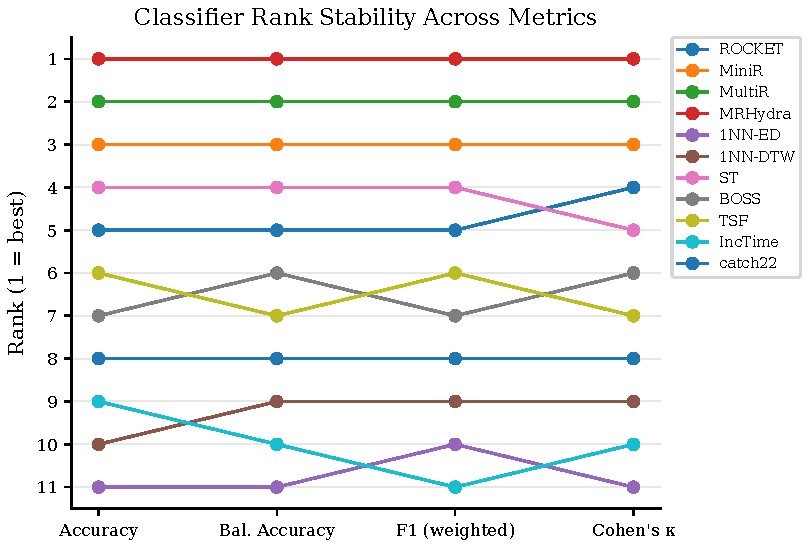
\includegraphics[width=\linewidth]{metric_rank_stability.pdf}
\caption{Classifier ranks across different evaluation metrics, demonstrating the stability of the top-performing models.}
\label{fig:rank_stability}
\end{figure}

\begin{table*}[t]
\centering
\caption{Mean classification accuracy ($\pm$ std) across 5 folds. \textbf{Bold} marks the best result per dataset.}
\label{tab:accuracy}
\begin{tabular}{lccccccccccc}
\toprule
Dataset & \rotatebox{60}{1NN-DTW} & \rotatebox{60}{1NN-ED} & \rotatebox{60}{BOSS} & \rotatebox{60}{InceptionTime} & \rotatebox{60}{MiniROCKET} & \rotatebox{60}{MultiROCKET} & \rotatebox{60}{MultiROCKETHydra} & \rotatebox{60}{ROCKET} & \rotatebox{60}{ST} & \rotatebox{60}{TSF} & \rotatebox{60}{catch22} \\
\midrule
Beef & 0.533 & 0.617 & 0.750 & 0.217 & \textbf{0.917} & 0.917 & 0.917 & 0.900 & 0.833 & 0.800 & 0.633 \\
CBF & 0.999 & 0.988 & \textbf{1.000} & 1.000 & 1.000 & 1.000 & 1.000 & 1.000 & 1.000 & 1.000 & 0.995 \\
Chinatown & 0.967 & 0.964 & 0.959 & 0.981 & 0.986 & \textbf{0.989} & 0.989 & 0.983 & 0.967 & 0.981 & 0.953 \\
Computers & 0.710 & 0.576 & 0.832 & 0.872 & 0.832 & 0.884 & \textbf{0.888} & 0.866 & 0.810 & 0.770 & 0.792 \\
ECG200 & 0.825 & 0.885 & 0.905 & 0.810 & 0.920 & 0.925 & 0.925 & \textbf{0.930} & 0.905 & 0.900 & 0.815 \\
EMOPain & 0.956 & 0.949 & -- & \textbf{0.970} & 0.943 & 0.933 & 0.937 & 0.854 & 0.862 & 0.924 & 0.914 \\
Earthquakes & 0.733 & 0.714 & 0.792 & 0.790 & 0.740 & 0.779 & 0.777 & \textbf{0.798} & 0.794 & 0.796 & 0.783 \\
EthanolLevel & 0.273 & 0.282 & 0.570 & 0.556 & 0.702 & 0.769 & 0.758 & 0.666 & \textbf{0.886} & 0.714 & 0.397 \\
MiddlePhalanxOutlineCorrect & 0.739 & 0.799 & 0.788 & 0.857 & 0.860 & 0.855 & \textbf{0.866} & 0.850 & 0.850 & 0.811 & 0.797 \\
SwedishLeaf & 0.817 & 0.829 & 0.935 & 0.976 & 0.978 & 0.982 & \textbf{0.986} & 0.972 & 0.952 & 0.916 & 0.900 \\
SyntheticControl & 0.992 & 0.923 & 0.975 & 0.997 & 0.983 & \textbf{0.998} & 0.997 & 0.998 & 0.995 & 0.988 & 0.990 \\
Trace & \textbf{1.000} & 0.820 & 1.000 & 0.890 & 1.000 & 1.000 & 1.000 & 1.000 & 1.000 & 1.000 & 1.000 \\
TwoPatterns & \textbf{1.000} & 0.986 & 1.000 & 1.000 & 1.000 & 1.000 & 1.000 & 1.000 & 0.999 & 0.997 & 0.877 \\
Worms & 0.608 & 0.512 & 0.736 & 0.492 & 0.771 & 0.771 & \textbf{0.787} & 0.717 & 0.756 & 0.674 & 0.751 \\
WormsTwoClass & 0.717 & 0.647 & \textbf{0.860} & 0.469 & 0.787 & 0.810 & 0.814 & 0.779 & 0.783 & 0.733 & 0.810 \\
\midrule
\textit{Avg. Accuracy} & 0.791 & 0.766 & 0.864 & 0.792 & 0.895 & 0.907 & \textbf{0.909} & 0.888 & 0.893 & 0.867 & 0.827 \\
\textit{Avg. Rank} & 8.17 & 9.47 & 6.67 & 6.27 & 4.63 & 3.27 & \textbf{2.93} & 4.53 & 5.50 & 6.57 & 8.00 \\
\bottomrule
\end{tabular}
\end{table*}


\subsection{Statistical Analysis}
We ran a Friedman test, which rejected the null hypothesis of equal classifier performance ($\chi^2 = 58.22$, $p < 10^{-6}$) and followed up with Post-hoc Nemenyi tests (CD $= 3.90$, $\alpha = 0.05$), which show that MultiROCKETHydra and MultiROCKET significantly outperformed the distance-based baselines (1NN-DTW, 1NN-ED) and catch22. However, no significant differences were found among the best performing classifiers (MultiROCKETHydra, MultiROCKET, ROCKET, MiniROCKET, ST). This indicates that the ROCKET family and ST form a statistically indistinguishable group in our experimentation. The critical difference diagram visualizes these groups.

\begin{figure}[htbp]
\centering
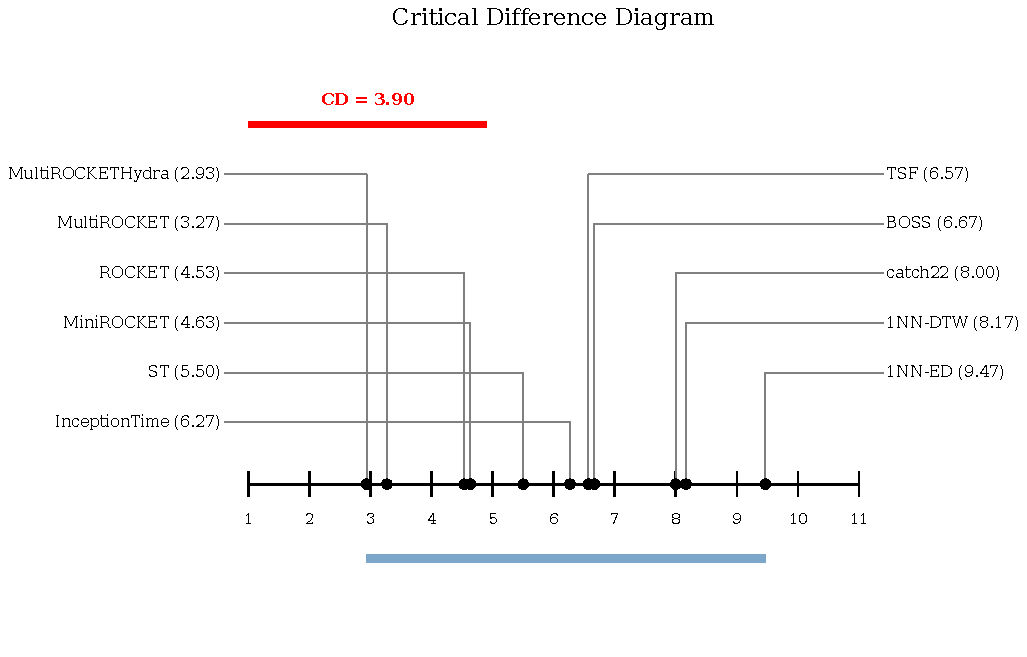
\includegraphics[width=\linewidth]{cd_diagram.pdf}
\caption{Critical Difference diagram showing the relative performance and statistical significance of the evaluated classifiers.}
\label{fig:cd_diagram}
\end{figure}

Since BOSS does not support multivariate time series, we penalized it by assigning it the last rank for the EMOPain dataset (30 channels, see Table~\ref{tab:datasets}).

\subsection{Computational Cost}
Training and inference time varied immensely with the different algorithms. The 1NN benchmark algorithms had the lowest fit times, but 1NN-DTW had by far the highest inference time. BOSS (639.4s) had the longest training time. The ROCKET family has the best tradeoff between accuracy and efficiency. MiniROCKET was the fastest algorithm of the ROCKET family (1.5s fit, 0.17s predict). We note that we plot the time consumption graphs on a log scale.

\begin{figure}[htbp]
\centering
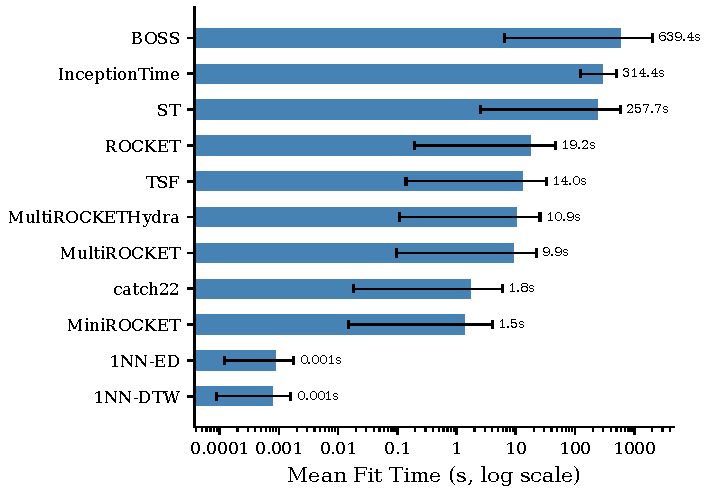
\includegraphics[width=0.8\linewidth]{fit_time_barplot.pdf}
\caption{Comparison of fit (training) times for the evaluated classifiers.}
\label{fig:fit_time}
\end{figure}

\begin{figure}[htbp]
\centering
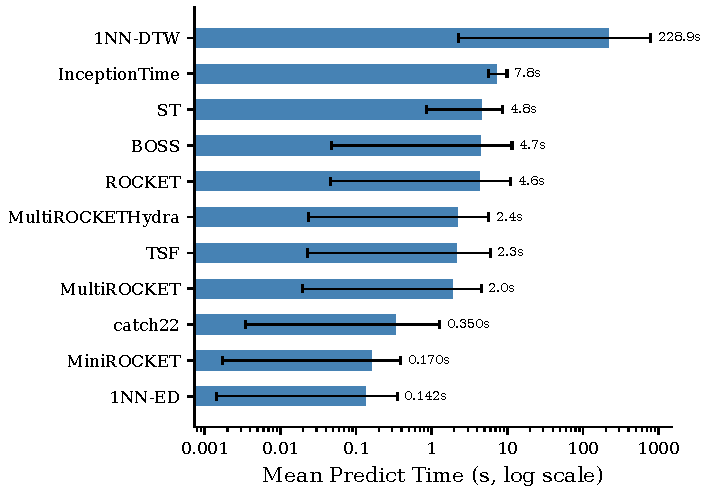
\includegraphics[width=0.8\linewidth]{predict_time_barplot.pdf}
\caption{Comparison of predict (inference) times for the evaluated classifiers.}
\label{fig:predict_time}
\end{figure}

\begin{figure}[htbp]
\centering
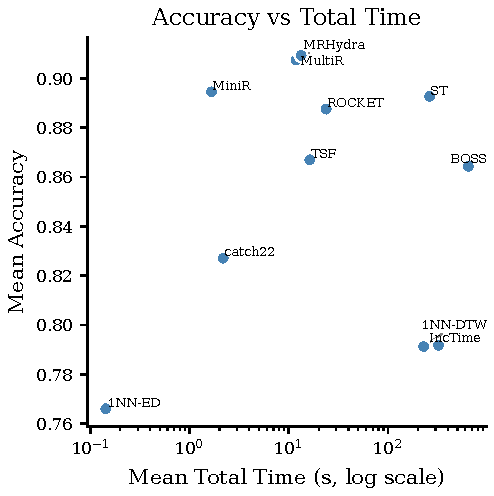
\includegraphics[width=\linewidth]{accuracy_vs_time_scatter.pdf}
\caption{Trade-off between classification accuracy and total computational time.}
\label{fig:acc_vs_time}
\end{figure}

\section{Conclusion}
In this paper, we evaluated the ROCKET algorithm and its recent variants—MiniROCKET, MultiROCKET, and Hydra—against a diverse suite of state-of-the-art benchmarks across 15 datasets from the UCR archive. Our results demonstrate that the ROCKET family consistently achieves a superior balance of classification accuracy and computational efficiency. Specifically, MultiROCKET and Hydra-MultiROCKET emerged as the top-performing models, achieving the highest mean accuracy and statistical significance over traditional distance-based and interval-based methods.

The experimental data confirms that ROCKET's reliance on random convolutional kernels provides a sufficiently rich feature space to match the performance of complex deep learning models like InceptionTime, while requiring orders of magnitude less training time. Furthermore, the scalability demonstrated in our time-complexity analysis suggests that ROCKET is uniquely suited for industrial applications involving high-frequency or large-scale sequential data where traditional ensemble methods become computationally prohibitive.

While ROCKET remains a "black-box" approach compared to shapelet-based methods, its near-deterministic variants like MiniROCKET provide a path toward stable, high-speed deployment. Future work will focus on improving the interpretability of the random kernels and extending the Hydra-MultiROCKET framework to more complex multivariate sensor fusion tasks.

\begin{thebibliography}{00}
\bibitem{b1} Dempster, A., Schmidt, D. F., and Webb, G. I. (2021). MiniROCKET: A Very Fast (Almost) Deterministic Transform for Time Series Classification. In Proceedings of the 27th ACM SIGKDD Conference on Knowledge Discovery and Data Mining.
\end{thebibliography}

\end{document}